
%\begin{enumerate}[label=\alph*)]
%\end{enumerate}

%\begin{definice}
%\end{definice}

%\sloppy

%\begin{poznamka}
%\end{poznamka}

%\begin{subequations}
%	\begin{align}
%	\end{align}
%\end{subequations}

%\begin{priklad}
%\end{priklad}

%\begin{veta}
%\end{veta}

%\begin{proof}
%\end{proof}

%\begin{figure}[!h]
%	\begin{center}
%		\includegraphics*[scale=0.9]{obr/krivka2}
%	\end{center}
%	\caption[caption]{\centering B-spline křivka stupně 2 (modře) a její řídící polygon (černě)\linebreak pro $U=\left\lbrace 0,0,0,1/4,1/2,3/4,3/4,1,1,1\right\rbrace $}
%	\label{obrKrivka}
%\end{figure}

%\begin{algorithm}[H]
%	\caption{Generování uzlového vektoru}
%	\label{GenKnotVec}
%	\begin{algorithmic}[1]
%		\Function{GenerateKnotVector}{$n,p$}
%		\State $j=1$;
%		\For{$i=0,\dots,n+p+2$}
%		\If{$(i\leq p)$}
%		\State $\text{knotVector}\left[i\right]=0$;
%		\ElsIf{$(i\leq n)$}
%		\State $\text{knotVector}\left[i\right]=j/\left(n-p+1\right)$;
%		\State $j\text{++}$;
%		\Else
%		\State $\text{knotVector}\left[i\right]=1$;
%		\EndIf
%		\EndFor
%		\State \textbf{return} knotVector;
%		\EndFunction
%	\end{algorithmic}
%\end{algorithm}

%\begin{subequations}
%	\begin{gather}
%	\end{gather}
%\end{subequations}

%\begin{equation}
%s=
%\begin{cases}
%\end{cases}
%\end{equation}

\clearpage
\chapter{Plánování cesty}
Nutnou podmínkou pro fungování autonomního robota je jeho navigace, která se skládá ze tří procesů:
\begin{enumerate}
	\item Lokalizace -- schopnost robota určit svoji polohu a orientaci v prostředí. Odpovídá na otázku "Kde se nacházím?"
	\item Mapování -- uložení dat získaných ze senzorů robota při prozkoumávání prostředí do dané reprezentace. Dává odpověď na otázku "Jak vypadá okolní svět?".
	\item Plánování cesty -- Proces nalezení posloupnosti akcí, které vedou k dosažení daného cíle. Jedná se o otázku "Jak se dostanu do cílové pozice?".
\end{enumerate}
Lokalizace a mapování jsou navzájem provázané -- při lokalizaci robota v prostředí je nutné znát jeho reprezentaci a pro správné mapování je nutné znát současnou polohu, ze které byla daná data získána. Plánování cesty je s těmito procesy úzce spjato, jelikož hledáme cestu v závislosti na současné poloze a reprezentaci prostředí. \cite{Meyer2003,Stachniss2009,Koubaa20180406}

\section{Formulace problému plánování cesty}\label{sec:stateSpace}
\subsection{Stavový prostor}
Každou jedinečnou situaci, do které se robot v prostředí může dostat, nazveme \emph{stav} $x$. Je důležité aby stav obsahoval právě ty informace, které potřebujeme k vyřešení problému. Množina stavů (označovaných $x$) se nazývá \emph{stavový prostor} $X$. Aplikací \emph{akce} $u$ na daný stav $x$ přejdeme do stavu $x'$, což je dáno tzv. \emph{přechodovou funkcí} $f$,
\begin{equation}
x'=f\left(x,u\right).
\end{equation}
Množinu $U(x)$, která reprezentuje všechny možné akce proveditelné ve stavu $x$ nazveme \emph{akčním prostorem}. Můžeme také definovat množinu všech možných akcí ve všech stavech jako
\begin{equation}
U=\bigcup_{x \in X} U(x).
\end{equation}
Dále definujeme množinu \emph{cílových stavů} $x_G \subset X$. Cílem obecného problému plánování je nalézt konečnou posloupnost akcí, která převede počáteční stav $x_0$ na některý z cílových stavů z $X_G$. 

Tento problém je možné interpretovat jako \emph{stavový přechodový graf}, ve kterém vrcholy reprezentují stavový prostor $X$ a orientovaná hrana grafu ze stavu $x$ do stavu $x'$ reprezentuje akci $u$ splňující funkci $x'=f(x,u)$. \cite{LaValle2006}

\subsection{Pracovní prostor}
Prostředí, ve kterém se robot pohybuje nazveme \emph{pracovní prostor} $W$. Jedná se o $N$-rozměrný Euklidovský prostor ($\mathbb{R}^2$ nebo $\mathbb{R}^3$). V pracovním prostoru se mohou vyskytovat různé překážky, ty značíme $O\subset W$. Překážky mohou být buď statické (nemění svoji polohu) nebo dynamické. \cite{Koubaa20180406}


\subsection{Konfigurační prostor}
Plánování cesty přímo v pracovním prostoru je z hlediska časové náročnosti velice neefektivní, jelikož stavový prostor je široký. Přináší také veliké problémy při zohlednění stupňů volnosti, různých tvarů a dalších mechanických omezení robota, které jsou pro různé aplikace odlišné. Pro zobecnění se používá tzv. \emph{konfigurační prostor} $C$.

V konfiguračním prostoru je robot reprezentován jako bod. \emph{Konfigurací} $q$ se myslí kompletní popis polohy a natočení robota v pracovním prostoru $W$. Konfigurační prostor $C$ je tedy množinou všech konfigurací $q$. Překážky $O$ vymezují \emph{kolizní konfigurační prostor} $C_{obs}$ tj. ty konfigurace, ve kterých by byl robot v kolizi s překážkou. Tzv. \emph{volný konfigurační prostor} je potom množinou všech přípustných konfigurací $C_{free}=C \setminus C_{obs}$. Nalezení \emph{přípustné cesty} je potom zobrazení
\begin{equation}
p: \left[0;L\right]\to C_{free},
\end{equation}
kde $L$ je délka cesty $p$. \cite{Koubaa20180406,Parker2009}

\subsection{Plánování cesty}

Problém plánování cesty lze tedy pomocí konfiguračního prostoru transformovat na problém hledání cesty ve stavovém přechodovém grafu. Uzly grafu jsou přípustné konfigurace $c\in C_{free}$. Každá hrana (tj. akce, přechod mezi danými konfiguracemi) má danou cenu. \cite{Ferguson2005}

Je důležité brát v potaz účel daného robota, jelikož různé aplikace mohou mít různé požadavky. Ve většině případů se jedná o optimalizaci ujeté vzdálenosti (tj. hledání nejkratší cesty). Dále je nutné dbát na účinnost, přesnost a bezpečnost robota i ostatních členů prostředí. Hledáme tedy ideálně cestu, při které se vyhneme kolizi s překážkami a dostaneme se do cíle v co nejkratším čase a za použití co nejméně energie. \cite{Koubaa20180406}

%Cílem plánování cesty je nalézt cestu z dané startovací pozice do cíle a při tom se vyhnout kolizi s překážkami. Zároveň je cílem optimalizovat nějakou kriteriální funkci, většinou uraženou vzdálenost, čas strávený cestou nebo co nejnižší energetický výdaj. [07342773;05585236;Liang15] 


\section{Plánování cesty pro více robotů}\label{sec:multirobotPathPlanning}
Výše byl definovaný problém plánování cesty robota, ze kterého vycházíme při definici problému plánování cesty pro více robotů. Obecně se jedná o situaci, kdy máme $m$ robotů v $k$-rozměrném pracovním prostoru a každý robot má danou startovní a cílovou konfiguraci, tj. pozici a orientaci. Je požadováno nalezení cesty pro každého robota, při které se budou roboti vyhýbat překážkám i sobě navzájem. \cite{Yu20140122}

Případy využití několika robotů současně jsou stále častější. Jedná se jak o použití v přepravě, průmyslu, zemědělství, rybaření, těžbě např. dřeva, hledání ztracených osob, prohledávání neznámých planet nebo likvidace toxického odpadu, tak o vojenské využití -- řízení bezpilotních letounů, pokládání nebo zneškodnění min, atd. \cite{Dudek1996}

Využití několika robotů může mít oproti použití pouze jednoho robota několik potenciálních výhod \cite{Dudek1996,Yan20130104}:
\begin{itemize}
	\item Prostorové rozložení -- vykonání úkonů v rozlehlých pracovních prostorech, které přesahují možnosti jednoho robota. Např. odpálení rakety otočením dvou klíčů současně.
	\item Celkový výkon systému -- systém několika robotů může lépe optimalizovat cenovou funkci jako např. čas potřebný k vykonání úkolu nebo celkovou energii spotřebovanou roboty.
	\item Sdílení informací -- např. více robotů je lépe schopno se lokalizovat navzájem, pokud si vyměňují informace.
	\item Cena -- použití několika jednoduchých (levnějších) robotů, které lze snadněji naprogramovat, může být levnější než použití jednoho komplexního (drahého) robota.
	\item Spolehlivost, flexibilita -- při selhání jednoho robota jej může nahradit další.
\end{itemize}


Úlohy plánování cesty pro více robotů lze rozdělit do několika skupin podle různých kriterií 
\cite{Koubaa20180406,Yu20140122,Asma2017,Solovey20160408,Silver2005,Alajlan2013}:
\begin{enumerate}
	%\item Podle úplnosti
	%\begin{enumerate}
		%\item \emph{Úplné} -- vždy naleznou cestu (pokud existuje) nebo ověří, že neexistuje. Časová náročnost těchto algoritmů však roste exponenciálně s počtem robotů.
		%\item \emph{Heuristické} -- nemusí nalézt žádnou cestu, i když existuje.
	%\end{enumerate}
	\item Podle typů jednotlivých robotů
	\begin{enumerate}
		\item \emph{Homogenní} -- schopnosti robotů jsou identické.
		\item \emph{Heterogenní} -- schopnosti robotů jsou různé. Každý robot má vlastní specializaci pro daný úkol. Obecně se jedná o náročnější plánování.
	\end{enumerate}
\clearpage
	\item Podle vzájemného chování robotů
	\begin{enumerate}
		\item \emph{Kooperativní} -- každý robot zná plány všech ostatních robotů. Roboti pracují společně na společném cíli. Speciálním případem je skupina mobilních robotů, která musí zachovávat předem určenou formaci, např. sekání fotbalového hřiště nebo přenášení nějakého předmětu více roboty.
		\item \emph{Nekooperativní} -- roboti neznají plány ostatních robotů a musí tak předvídat jejich pohyby.
		\item \emph{Antagonistické} -- každý robot se snaží dosáhnou svého cíle a případně zamezit ostatním robotům v dosažení jejich cílů.
	\end{enumerate}
	\item Podle povahy prostředí
	\begin{enumerate}
		\item \emph{Statické} -- obsahuje pouze překážky, které nemění svoji polohu.
		\item \emph{Dynamické} -- obsahuje pohybující se překážky (např. lidé).
	\end{enumerate}
	\item Podle znalosti prostředí
	\begin{enumerate}
		\item \emph{Globální plánování cesty} -- roboti mají úplnou znalost pracovního prostoru před plánováním cesty.
		\item \emph{Lokální plánování cesty} -- roboti mají neúplnou nebo žádnou znalost okolního prostředí. Musejí tedy v reálném čase snímat pomocí senzorů polohu překážek, vytvářet mapu prostředí a hledat v ní cestu.
	\end{enumerate}
	\item Podle času provádění plánování
	\begin{enumerate}
		\item \emph{Offline} -- nejdříve je provedeno plánování cesty pro všechny roboty, poté se roboti podle těchto plánů začnou pohybovat.
		\item \emph{Online}, příp. \emph{real-time} -- plánování cesty je spojeno s pohybem robotů. Nalezená cesta nemusí být optimální nebo vůbec nalezena, roboti ale netráví dlouhý čas plánováním a dokáží rychle reagovat i na změny prostředí.
	\end{enumerate}
	\item Podle přístupu k řešení problému
	\begin{enumerate}
		\item \emph{Centralizované} -- bere v úvahu všechny roboty zároveň jako jeden propojený systém. Snaží se o optimalitu a úplnost, proto v praxi trpí velikou časovou náročností.
		\item \emph{Distribuované} -- rozdělí plánování na menší nezávislé nebo slabě závislé problémy, které řeší každý robot zvlášť. Schopné rychle nalézt dobré řešení, avšak ztrácí na úplnosti.
	\end{enumerate}
\end{enumerate}

\section{Zpracování prostředí}
Pro zobecnění problému plánování cesty robota do prohledávání v konfiguračním prostoru $C$ je nutná vhodná reprezentace prostředí, ve kterém se robot pohybuje. Jak uvádí například \cite{LaValle2006,Masehian2007}, existuje několik přístupů ke zpracování prostředí, kdy k nejznámějším například patří \textit{mapy cest}, \textit{rozklad do buněk} nebo \textit{potenciálová pole}.

\subsection{Mapy cest (Roadmaps)}
Přístup ke zpracování prostředí pomocí map cest je založen na myšlence, že prostor $C$ je zredukován či zmapován do sítě jednodimenzionálních křivek, které neprotínají překážky. Hledání řešení je poté omezeno na tuto síť a problém plánování cesty se stává problémem prohledávání grafu. Rozlišujeme dvě základní skupiny, a to \textit{deterministické} a \textit{pravděpodobnostní} metody.
\begin{enumerate}
	\item \textbf{Deterministické metody}
	\begin{enumerate}
		\item \textbf{Voroného diagramy}\\
		Jedná se o metodu rozdělení prostoru podle určité množiny objektů (v našem případě například překážek). Voroného diagram je potom množina všech bodů, které jsou stejně vzdálené od dvou nebo více objektů. Tento diagram poté rozděluje prostor do oblastí, které obsahují právě jeden objekt. Cesta v tomto diagramu poté není nutně nejkratší, ale udává maximální možnou vzdálenost od překážek. \cite{Yan20130104,Opfer20111202} Na obrázku \ref{obr:voronoi} můžeme vidět příklad Voroného diagramu.
		%Voroného diagram každému bodu $x$ z určité množiny $M$ přidělí oblast $V(x)$ tak, aby všechny body této oblasti byly blíže k bodu $x$ než k jakémukoliv jinému bodu z množiny $M$ \cite{monografie5}, viz obrázek \ref{voro}.
		\begin{figure}[h!]
			\begin{center}
				\includegraphics*[width=15cm,height=7cm,keepaspectratio]{obr/voronoi}
			\end{center}
			\caption{Voroného diagram 14 bodů v rovině \cite{Opfer20111202}}
			\label{obr:voronoi}
		\end{figure}
	
		\item \textbf{Graf viditelnosti}\\
		Vrcholy grafu viditelnosti jsou tvořeny vrcholy překážek a startovací a cílovou pozicí. Hrany grafu jsou pak spojnice těch vrcholů, jejichž spojnice neprotíná žádnou překážku. Tvar překážek je omezen na polygon. Příklad grafu viditelnosti je zobrazen na obrázku \ref{obr:visibilityGraph}.
		
		\begin{figure}[h!]
			\begin{center}
				\includegraphics*[width=15cm,height=7cm,keepaspectratio]{obr/visibilityGraph}
			\end{center}
			\caption{Graf viditelnosti \cite{Tsourdos2010}}
			\label{obr:visibilityGraph}
		\end{figure}
		
%		V případě odstranění těch hran, jejichž prodloužení je ve volném prostoru, se jedna o graf tečen \cite{monografie3}, viz obrázek \ref{tecny}.
%		
%		\begin{figure}[h!]
%			\begin{center}
%				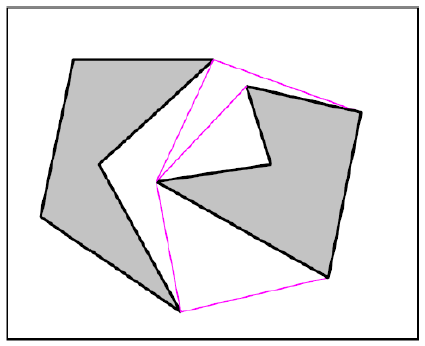
\includegraphics[scale=0.7]{obr/tecny}
%			\end{center}
%			\caption{Graf tečen \cite{monografie3}}
%			\label{tecny}
%		\end{figure} 
	\end{enumerate}
	\item \textbf{Pravděpodobnostní metody}
	\begin{enumerate}
		\item \textbf{Pravděpodobnostní mapy cest}\\
		Tato metoda náhodně generuje a propojuje velké množství bezkolizních konfigurací z volného konfiguračního prostoru $C_{free}$. Plánování cesty poté probíhá v takto vytvořeném grafu.
		
		\begin{figure}[h!]
			\begin{center}
				\includegraphics*[width=15cm,height=6cm,keepaspectratio]{obr/probRoadMap}
			\end{center}
			\caption{Příklad pravděpodobnostní mapy cest \cite{LaValle2006}}
			\label{obr:probRoadMap}
		\end{figure}
		
		\item \textbf{Pravděpodobnostní stromy}\\
		Jedná se o metodu, kdy se postupně vytváří stromová struktura, která rychle prorůstá prostředím. Jedná se například o Rapidly-exploring Random Tree (RRT, rychle rostoucí náhodný strom), kde je konstrukce stromu náhodná -- náhodná konfigurace z volného konfiguračního prostoru $C_{free}$ je připojena k nejbližší konfiguraci, která je součástí stromu. Příklad můžeme vidět na obrázku \ref{obr:RRT}. Tato metoda je velice efektivní, s rostoucím počtem iterací roste pravděpodobnost dosáhnutí libovolného bodu v prostoru, která se limitně blíží $1$. \cite{LaValle2006}
		
		\begin{figure}[h!]
			\begin{center}
				\includegraphics*[width=15cm,height=6cm,keepaspectratio]{obr/RRT}
			\end{center}
			\vspace*{4mm}
			\caption{RRT po 45 iteracích (vlevo) a po 2345 iteracích (vpravo) \cite{LaValle2006}}
			\label{obr:RRT}
		\end{figure}
	\end{enumerate}
\end{enumerate} 

\subsection{Rozklad do buněk (Cell decomposition)}
V metodě rozkladu do buněk je prostředí rozděleno na nepřekrývající se
buňky. U každé buňky se určí, jestli obsahuje překážku či ne a na základě toho se vytvoří graf, kde vrcholy tvoří buňky neobsahující překážku a hrany pak spojnice mezi nimi. Rozlišujeme dva základní rozklady a to \textit{aproximativní rozklad} a \textit{exaktní rozklad}.
	\begin{enumerate}
		\item \textbf{Exaktní rozklad}\\
		Pracovní prostor je rozložen do vzájemně nepřekrývajících se buněk různého tvaru. Mezi buňkami jsou umístěny body přechodu a nalezená cesta se pak skládá z počátečního stavu, ze kterého se jde skrze body přechodu do cílového stavu. Příklad exaktního rozdělení je na obrázku \ref{obr:exact}. \cite{LaValle2006}
		
		\begin{figure}[h!]
			\begin{center}
				\includegraphics*[width=15cm,height=6cm,keepaspectratio]{obr/exact}
			\end{center}
			\caption{Příklad exaktního rozkladu \cite{LaValle2006}}
			\label{obr:exact}
		\end{figure}
		
		\item \textbf{Aproximativní rozklad}\\
		Pracovní prostor je rozdělen do buněk stejného tvaru -- většinou se jedná o čtverce, ale je možné použít také například šestiúhelníky nebo trojúhelníky. Důležitou částí aproximace prostředí do této podoby je vhodná volba velikosti buněk. Čím menší velikost buněk použijeme, tím je rozklad přesnější, nicméně za cenu zvýšené výpočetní a paměťové náročnosti. Každá buňka je buď průchozí nebo neprůchozí, obsahuje-li alespoň část překážky. Příklad aproximativního rozkladu je zobrazen na obrázku \ref{obr:aprox} -- vybarvené buňky obsahují překážky, jsou tedy označené za neprůchozí. \cite{Abd Algfoor2015}
		%Buňky jsou rozdělené do dvou skupin a to na volné buňky a obsazené. Obsazené buňky jsou všechny buňky, které alespoň trochu obsahují překážku. Což vede na problém, kdy buňka obsahuje opravdu jen malou část překážky a zbytek buňky je volný ale musí být označený za obsazený a nemusí kvůli tomu být nalezená cesta. Tento problém je právě řešen užitím menší velikosti buněk. 
		
		\begin{figure}[h!]
			\begin{center}
				\includegraphics*[width=15cm,height=6cm,keepaspectratio]{obr/aprox}
			\end{center}
			\caption{Příklad aproximativního rozkladu \cite{Tsourdos2010}}
			\label{obr:aprox}
		\end{figure}
		
	\end{enumerate}


\subsection{Potenciálová pole (Potential fields)}
%Metoda potenciálového pole bylo poprvé navržena v roce 1985. 
V tomto případě je robot reprezentován jako bod v konfiguračním prostoru a jako částice pod vlivem umělého potenciálového pole. Cílový stav má přiřazen pozitivní potenciál, kdežto překážky mají odpudivý potenciál. Myšlenka je taková, že robot pohybující se v potenciálovém poli bude přitahován k cíli, zatímco bude odpuzován překážkami. Na rozdíl od mapy cest a rozkladu do buněk, cesta nalezena touto metodou následuje linii maximálního potenciálu spojité funkce potenciálového pole. Hlavní výhodou je rychlý výpočet potenciálové funkce. Tato metoda má však určité nevýhody, hlavní je, že se robot může zachytit v lokálním minimu, například když
narazí na překážku ve tvaru písmene C. Další nevýhody jsou například oscilace v úzkých prostorech, případně úplné znemožnění cesty mezi blízkými objekty. Příklad potenciálového pole je na obrázku \ref{obr:potential}. \cite{Tsourdos2010,Wallar2014,Masehian2004}

\begin{figure}[h!]
	\begin{center}
		\includegraphics*[width=15cm,height=6cm,keepaspectratio]{obr/potential}
	\end{center}
	\caption{Potenciálové pole \cite{Opfer20111202}}
	\label{obr:potential}
\end{figure} 

%\subsection{Matematické programování} 
%Matematické programování je metoda hledání nejkratší cesty prostřednictvím řešení optimalizačního problému, který hledá cestu mezi startovací a cílovou pozicí minimalizací určitého skalár \cite{monografie2}.

%Pro zobecnění problému plánování cesty robota do prohledávání v konfiguračním prostoru $C$ je nutná vhodná reprezentace prostředí, ve kterém se robot pohybuje.
%\subsection{Rozklad do buněk (Cell decomposition)}
%\subsection{Mapy cest (Roadmaps)}
%Visibility graph, Voronoi diagram
%\subsection{Potenciálová pole (Potential fields)}

\section{Metody plánování cesty}
Po dokončení fází lokalizace a mapování (tj. zpracování prostředí) se pro plánování cesty mezi danou startovací a cílovou pozicí použijí konkrétní plánovací algoritmy. Výběr vhodného algoritmu je závislý na daném problému a jeho omezeních a požadavcích. Plánovacích algoritmů existuje mnoho, každý se svými specifiky, uvedeme si zde proto nejvíce používané přístupy. Můžeme je rozdělit např. podle kriterií uvedených v podkapitole \ref{sec:multirobotPathPlanning}, případně je dělíme na tzv. metody klasické a metody umělé inteligence.

\subsection{Klasické metody}
Jak bylo řečeno v podkapitole \ref{sec:stateSpace}, lze stavový prostor interpretovat jako graf, kde vrcholy představují všechny možné konfigurace robotů a hrany přechody mezi nimi.
Cílem je najít takovou posloupnost přechodů mezi těmito stavy takovou, aby se každý robot dostal z výchozí pozice do pozice cílové a aby se minimalizovala nějaká celková cenová funkce.

Obecně je problém plánování cesty pro více robotů NP-úplný. Metody, které tento problém řeší lze tedy rozdělit do dvou skupin:
\begin{enumerate}
	\item \emph{úplné} -- vždy naleznou cestu (pokud existuje) nebo ověří, že neexistuje. %Časová náročnost těchto algoritmů však roste exponenciálně s počtem robotů.
	\item \emph{neúplné} -- nemusí nalézt žádnou cestu, i když existuje.
\end{enumerate}
Vybrané neúplné metody budou představeny v kapitole \ref{sec:algos}, zde tedy představíme některé metody úplné, jak je popisují \cite{Goldenberg2012,STANDLEY,Kraft2017}.

\subsubsection{Grafové algoritmy}
Řešení lze nalézt pomocí některého grafového algoritmu, např. Dijkstrův \cite{Dijkstra1959} nebo A* (viz podkapitola \ref{sec:Astar}). Uvažujeme-li prostředí reprezentované osmisměrnou mřížkou, má každý robot k dispozici 9 akcí (8 směrů + čekat). Pro $n$ robotů je v každém kroku tedy možných až $9^n$ akcí. I když pro triviální případy je možné tento přístup využít, s rostoucím počtem robotů roste časová složitost i nároky na paměť exponenciálně.

\subsubsection{Pattern databases}
Pro některé problémy mohou být klasické heuristické funkce nedostatečné. Je možné využít techniky \emph{Pattern database}, kdy se předem spočítají vzdálenosti do cíle v abstraktním stavovém prostoru (kde neuvažujeme některá omezení nebo proměnné). Tyto hodnoty jsou poté použity při hledání jako odhady vzdáleností v původním stavovém prostoru.

\subsubsection{Operator Decomposition}
Při expandování uzlů z fronty $open$ dochází ke generování velkého počtu dalších uzlů, které nakonec nemusejí být ani použity. Pro redukci tohoto množství je možné použít metodu \emph{Operator decomposition}. V této metodě jsou při expanzi uzlu brány v potaz pouze sousední stavy prvního robota, které se nazývají \emph{přechodné}. Tyto stavy vkládáme normálně do fronty $open$, ale při jejich expanzi jsou brány v potaz pouze možné akce dalšího robota. Při expanzi uzlu posledního robota jsou generovány tzv. \emph{standartní} uzly. Pouze tyto standartní uzly tvoří výslednou cestu. 

\subsubsection{Independence Detection}
Často je počet robotů malý oproti velikosti pracovního prostoru, případně je jen málo míst kde by mohlo dojít ke kolizi mezi roboty. Není tedy nutné provádět hledání pro všechny roboty současně, ale můžeme vyhledat cestu pro každého zvlášť a poté zkontrolovat, jestli jsou nalezené cesty kolizní. Metoda \emph{Independence Detection} rozdělí roboty do \emph{nezávislých} skupin, tj. skupin, jejichž cesty nevedou ke kolizi. Nejprve je každý robot sám ve vlastní skupině. Pro každou skupinu je nalezena nejkratší cesta a simulován pohyb po této cestě (pro všechny skupiny současně). Pokud dojde ke konfliktu, je buď upravena cesta kolizních skupin nebo jsou tyto skupiny sloučeny. Tento proces se opakuje dokud nenalezneme bezkonfliktní cestu pro všechny skupiny. Celkový čas hledání je potom závislý na času hledání cesty největší skupiny. 

\begin{figure}[h!]
	\begin{center}
		\includegraphics*[width=15cm,height=7cm,keepaspectratio]{obr/independenceDetection}
	\end{center}
	\caption{Příklad hledání pomocí Independence Detection \cite{Kraft2017}}
	\label{obr:independenceDetection}
\end{figure}

\subsubsection{Partial Expansion A*}
Další metodou pro redukci velikosti prioritní fronty $open$ je \emph{Partial Expansion A*} (PEA*). Při expanzi uzlu $n$ jsou do prioritní fronty vloženy pouze ty uzly, pro které platí $f\leq f(n)$. Uzel $n$ je opět vložen do fronty s hodnotou $f$ rovnou nejnižší hodnotě $f$ z expandovaných uzlů. Výhodou je tedy omezený počet uzlů ve frontě $open$ a tedy i její nižší paměťová náročnost. Nevýhodou je ovšem opětovné expandování a generování uzlů, čímž může narůst časová náročnost algoritmu.

\emph{Enhanced Partial Expansion A*} staví na PEA*, využívá znalosti fungování použité heuristiky a snaží se minimalizovat čas potřebný k opětovnému expandování uzlů. Například při použití Manhattanské metriky dopředu víme, pro které uzly se hodnota $h$ zvýší nebo sníží, v závislosti na poloze cílového uzlu. Tím je dosažena nejen paměťová, ale i časová úspora. Nevýhodou je ovšem nemožnost použití složitější heuristiky, jako např. Pattern database.

%\subsubsection{Hierarchical A*}
 

\subsection{Metody umělé inteligence}
Klasické metody mají několik hlavních nevýhod, především velkou časovou náročnost při vyšších dimenzích. Nabízí se využití některých meta-heuristik, které pomáhají při řešení optimalizačních problémů. I když tyto algoritmy nejsou úplné (tj. negarantují nalezení řešení), bývají často mnohem rychlejší než metody úplné. Kromě zde popsaných algoritmů patří mezi metody umělé inteligence například neuronové sítě, simulované žíhání, Tabu search nebo fuzzy logika. Konkrétní varianty těchto algoritmů pro řešení problému plánování cesty můžeme nalézt v \cite{Masehian2007}.


\subsubsection{Inteligence hejna}
Inteligence hejna (SI -- Swarm Intelligence) je systém kolektivního chování jednoduchých agentů, kteří spolu a se svým okolím lokálně interagují. Toto chování, i když není centrálně řízené, dává vzniknout složitému globálnímu chování hejna. Je to koncept založený na sociálním chování mravenců, ryb, ptáků, včel, světlušek atd. Podrobnější popis těchto algoritmů včetně srovnání jejich výhod a nevýhod se nachází v článku \cite{SinghPal20131218}.

\begin{enumerate}
	\item \textbf{Optimalizace hejnem částic}\\
	Optimalizace hejnem částic (PSO -- Particle Swarm Optimization) poprvé popsali ve svém článku Kennedy a Eberhart v roce 1995 \cite{Kennedy1995}. Jedná se o evoluční meta-heuristickou techniku inspirovanou sociálním chováním hejna ptáků při hledání potravy, uplatněním vzájemného sdílení informací. Toto chování je simulováno populací částic, kde každá částice představuje jedno konkrétní řešení. Tyto částice jsou náhodně rozmístěny ve stavovém prostoru, který postupně prohledávají a hledají optimální řešení nebo alespoň řešení blízko optimálnímu. Každá částice má danou polohu $P$ a vektor rychlosti $v$. V každé iteraci je vyhodnocena současná pozice částice pomocí tzv. \emph{účelové funkce} a pokud je tato hodnota lepší než dosud nalezená, je uložena jako $P_{best}$. Nejlepší hodnota všech částic je uložena jako $G_{best}$. Dále je spočítána další pozice částice a její rychlost pomocí rovnic
	\begin{subequations}
		\begin{align}
		v_{i+1}&=wv_i+c_1r(P_{best}-P_i)+c_2r(G_{best}-P_i),\\
		P_{i+1}&=P_i+v_{i+1},
		\end{align}
	\end{subequations}
	kde $r$ je náhodné číslo v intervalu $(0,1)$, $w$ je setrvačnost částice a $c_1,c_2$ jsou akcelerační koeficienty. Podmínka ukončení je většinou počet iterací nebo minimální požadovaná odchylka od minima.
	
	Jednou z největších nevýhod je předčasná konvergence algoritmu, tj. možnost uvíznutí v lokálním optimu. Další nevýhodou je velká náchylnost na dané parametry, které jsou pro každý problém různé. PSO a jeho varianty se nejčastěji uplatňují v problémech plánování cesty několika robotů, ve kterých skupina robotů prohledává neznámý prostor. \cite{Masehian2007,Asma2017,Nakisa20140901}
	
	\item \textbf{Optimalizace mravenčí kolonií}\\
	Optimalizace mravenčí kolonií (ACO -- Ant Colony Algorithm) je další ze skupiny algoritmů inteligence hejna. Jak název napovídá, jedná se o metodu inspirovanou chováním mravenců při hledání potravy. Mravenci jsou schopni nalézt nejkratší cestu k potravě a zpět do mraveniště a reagovat na změny v prostředí, aniž by využívali vizuální informace. Sdílení informací mezi mravenci probíhá pomocí feromonové (chemické) stopy. Při pohybu mravenců dochází k uvolňování feromonů na zem, čímž se označí cesta. Feromony se postupen času odpařují. Čím více mravenců se pohybuje po stejné trase, tím více je tato cesta atraktivnější pro další mravence. Jedná se o pozitivní zpětnou vazbu, kdy pravděpodobnost, že mravenec zvolí danou cestu je přímo úměrná počtu mravenců, kteří touto cestou prošli. \cite{Liu2006}
	 
	 
	 \begin{figure}[h!]
	 	\begin{center}
	 		\includegraphics*[width=15cm,height=6cm,keepaspectratio]{obr/Aco_TSP}
	 	\end{center}
	 	\caption{ACO použité pro řešení problému obchodního cestujícího \cite{Dreo2006}}
	 	\label{obr:Aco_TSP}
	 \end{figure} 
	 
	\item \textbf{Umělá včelí kolonie}\\
	Umělou včelí kolonii (ABC -- Artificial Bee Colony) představil ve svém článku \emph{An idea based on honey bee swarm for numerical optimization} v roce 2005 Dervis Karaboga \cite{Karaboga2005}. Jedná se o metodu inspirovanou včelami hledajícími zdroje potravy v okolí úlu. Kolonie se skládá ze tří druhů včel: dělnice, vyčkávací včely a průzkumnice. Dělnice jsou vyslány ke zdroji nektaru, se kterým se poté vrací zpět do úlu. Poté prostřednictvím tance komunikují s ostatními včelami. Vyčkávací včely podle tohoto tance vyberou zdroje potravy, ke kterým se vydají. Pokud je tento zdroj vyčerpán, vyčkávací včely se stávají průzkumnicemi. Průzkumnice provádí náhodné hledání v okolí úlu. Zdroje potravy reprezentují řešení a množství jejich nektaru odpovídá jeho kvalitě (fitness funkce). \cite{SinghPal20131218}
	
	Výhodou ABC algoritmu je jeho jednoduchost, flexibilita a malé množství kontrolních parametrů, nevýhodou je nepřesnost nalezeného řešení a pomalá konvergence \cite{Liang2015}.
	
\end{enumerate}
\subsubsection{Genetické algoritmy}
John Holland poprvé předložil genetický algoritmus, založený na Darwinově teorii evoluce, již v roce 1960. Jedná se o náhodný prohledávací algoritmus, kde řešení problému je zakódováno do chromozomů. Nejprve je vytvořena počáteční populace, která je složená z náhodných členů (chromozomů). Pro každý chromozom je poté při každé iteraci spočtena tzv. \emph{fitness funkce}, která vyjadřuje kvalitu daného jedince. Podle této hodnoty jsou pomocí selekce vybráni další jedinci určení k reprodukci. Poté dochází ke křížení -- vzniku nových jedinců kombinací chromozomů dvou rodičů. Dále dochází k mutaci, kdy se mění genetická struktura některých jedinců. Tento cyklus se opakuje, dokud není splněna některá ukončovací podmínka, např. počet iterací nebo pokud se generace nevyvíjí dostatečně rychle. 

Jednou z hlavních výhod genetického algoritmu je jeho jednoduchá paralelizace, nevýhodou je potom možnost uvíznout v lokálním minimu a jeho pomalá konvergence. Genetický algoritmus je také hojně využíván v kombinaci s ostatními přístupy, jako A*, ACO, potenciálovými poly. \cite{Lamini2018,Masehian2007,Gao2008,Alajlan2013}


\clearpage
\chapter{Vybrané algoritmy}\label{sec:algos}

K implementaci byly v této diplomové práci zvoleny klasické metody, založené na grafových algoritmech. Plánování probíhá v konfiguračním prostoru získaném metodou rozkladu do buněk. Základním a nejpoužívanějším algoritmem pro hledání nejkratší cesty v grafu je A* algoritmus. Z něj vychází modifikace pro řešení problému plánování cesty pro více robotů popsaných v této kapitole.

\section{A* Algoritmus}\label{sec:Astar}
\emph{A* algoritmus} ve svém článku \emph{A formal basis for the heuristic determination of minimum cost paths} představili P. Hart, N. Nilsson a B. Raphael \cite{Hart1968}. Jeho vstupem je graf, který má ohodnocené hrany (tzv. \emph{ceny přechodu} z jednoho stavu do druhého), startovací a cílový stav. Výstupem je pak nejkratší cesta ze startovací do cílové pozice a nebo informace o tom, že taková cesta neexistuje. 

Algoritmus využívá prioritní frontu (zvanou \emph{OPEN}), ve které jsou jednotlivé stavy určené k expanzi seřazeny dle hodnoty \emph{hodnotící funkce} $f$. Tato funkce má tvar
\begin{equation}
	f\left(x\right) = h\left(x\right) + g\left(x\right),
\end{equation}
kde $ g\left(x\right)$ je funkce představující vzdálenost mezi počátečním stavem a aktuálním stavem a $h\left(x\right)$ je heuristická funkce, která představuje odhad vzdálenosti od aktuálního stavu do cílového stavu. Tato funkce musí být \emph{přípustná}, což znamená že nesmí nadhodnocovat vzdálenost k cílové pozici. Další vlastností, kterou může mít tato heuristická funkce, je monotónnost. Takovou vlastnost má funkce, pokud splňuje podmínku
\begin{equation}
	h\left(x\right)\leq d\left(x,y\right) + h\left(y\right),
\end{equation}
kde $d$ je cena přechodu mezi stavem $x$ a $y$. Pokud je tato vlastnost splněna, algoritmus navštíví každý uzel maximálně jednou.

Heuristická funkce může být libovolná, ale pro hledání nejkratší cesty je vhodné opírat se o teorii metrických prostorů. Zde představíme čtyři základní metriky a to \emph{euklidovskou}, \emph{manhattanskou}, \emph{Čebyševovu} a metriku \emph{octile}. \cite{Patel19972020}

\begin{itemize}
	\item \emph{Euklidovská metrika} je dána vztahem 
	\begin{equation}
	\rho_e\left(\vec{p},\vec{q}\right)=\sqrt{\sum_{i=1}^n\left(q_i-p_i\right)^2}
	\end{equation}
	a představuje jednoduše délku vzdušné spojnice mezi stavem $p$ a $q$, viz obr. \ref{obr:euclid}.
	
	\begin{figure}[htb]
		\begin{center}
			\includegraphics*[width=15cm,height=6cm,keepaspectratio]{obr/euclid}
		\end{center}
		\caption{Euklidovská metrika}
		\label{obr:euclid}
	\end{figure}
	
	\item \emph{Manhattanská metrika} je inspirovaná pravoúhlým systémem ulic na Manhattanu v New Yorku a je definovaná vztahem
	\begin{equation}
	\rho_m\left(\vec{p},\vec{q}\right)=\sum_{i=1}^n\left|q_i-p_i\right|
	\end{equation}
	Na obrázku \ref{obr:manhat} je zobrazen příklad manhattanské metriky, kde všechny cesty, ať už červená, modrá nebo žlutá mají stejnou délku. 
	
	\begin{figure}[htb]
		\begin{center}
			\includegraphics*[width=15cm,height=6cm,keepaspectratio]{obr/manhat}
		\end{center}
		\caption{Manhattanská metrika}
		\label{obr:manhat}
	\end{figure}

	\item \emph{Čebyševova (maximální) metrika} počítá pouze s nejdelší složkou vzdálenosti, tj. je daná vztahem
	\begin{equation}
	\rho_c\left(\vec{p},\vec{q}\right)=\max_{\forall i}\left|q_i-p_i\right|.
	\end{equation}
	Obrázek \ref{obr:chebyshev} ukazuje, že všechny sousední buňky mají v Čebyševově metrice vzdálenost 1.
	
	\begin{figure}[htb]
		\begin{center}
			\includegraphics*[width=15cm,height=6cm,keepaspectratio]{obr/chebyshev}
		\end{center}
		\caption{Čebyševova metrika}
		\label{obr:chebyshev}
	\end{figure}
	
	\item Octile metrika kombinuje pohyb  diagonální a přímý a mezi dvěma stavy (ve 2D mřížce) je definovaná jako
	\begin{equation} \rho_o\left(\vec{p},\vec{q}\right)=\max\left(\left|p_1-q_1\right|,\left|p_2-q_2\right|\right)+(\sqrt{2}-1)\cdot \min\left(\left|p_1-q_1\right|,\left|p_2-q_2\right|\right).
	\end{equation}
	Příklad octile metriky je zobrazen na obrázku \ref{obr:octile}.
	
	\begin{figure}[htb]
		\begin{center}
			\includegraphics*[width=15cm,height=6cm,keepaspectratio]{obr/octile}
		\end{center}
		\caption{Octile metrika}
		\label{obr:octile}
	\end{figure}
	
\end{itemize} 

Nyní k samotnému popisu algoritmu. Jak již bylo řečeno na začátku této podkapitoly, algoritmus pracuje s prioritní frontou (\emph{OPEN}) nenavštívených uzlů grafu. Uzly jsou seřazeny dle hodnoty funkce $f$ a čím nižší je její hodnota, tím vyšší má uzel prioritu. V každé iteraci je uzel s nejnižší hodnotou funkce $f$ odebrán a jsou spočítány hodnoty $g$  a $f$ jeho sousedních uzlů. V případě, že tyto uzly nejsou v prioritní frontě, tak jsou tam přidány, a pokud již ve frontě jsou, tak aktualizujeme hodnotu funkce $f$, pokud je nižší. Algoritmus pokračuje do té doby, dokud nenalezne koncový uzel nebo dokud nedojde k vyprázdnění fronty \emph{OPEN}. Hodnota $g$ koncového uzlu je pak hodnota nejkratší cesty ze startovacího uzlu do koncového. Tento postup je popsán v algoritmu \ref{alg:Astar}.

%\begin{figure}[htb]
%	\begin{center}
%		\includegraphics*[width=15cm,height=6cm,keepaspectratio]{obr/pr1}
%	\end{center}
%	\caption{Výchozí stav probému}
%	\label{pr1}
%\end{figure}
%
%Algoritmus si ukážeme na příkladu z obrázku \ref{pr1}. V prvním kroku je přidán do prioritní fronty startovací uzel, nejedná se o koncový uzel a tak výpočet pokračuje. Pro jeho sousední uzly $ A $ a $ B $ jsou vypočteny hodnoty funkce $ f $. Do prioritní fronty jsou přidány trojice [aktuální uzel, předchůdce, hodnota funkce $ f $]. Uzel $ S $ byl tedy expandován a nyní se odstraní z prioritní fronty do seznamu pro již expandované uzly. Momentálně prioritní fronta tedy obsahuje
%$$ OPEN = ([B, S, 4], [A, S, 7], [C, S, 11]).  $$
%V druhém kroku je vybrán uzel s nejmenší hodnotou funkce $ f $, což je v našem případě uzel $ B $. Ten má pouze jednoho následníka a to uzel $ D $. Pro něj je vypočtena hodnota funkce $ f = 8 $, je přidán do seznamu OPEN, ze kterého je odstraněn uzel $ B $, který je přidán do seznamu CLOSE. Prioritní fronta nyní obsahuje
%$$ OPEN = ([A, S, 7], [D, B, 8], [C, S, 11]).  $$
%V dalším kroku vybereme uzel $ A $, jehož následník je uzel $ C $, který už sice v prioritní frontě je, ale je potřeba zkontrolovat, jestli nová hodnota funkce $ f $ není menší. Hodnota funkce $ f $ je 12, což je větší jak stará hodnota a proto se nic nemění a jediné, co se děje je to, že je z fronty odebrán uzel $ A $. V další kroku je tedy vybrán uzel $ D $ opět s následníkem $ C $, jehož hodnota funkce $ f $ je nyní 9. Prioritní fronta nyní obsahuje pouze uzel $ C $ 
%$$ OPEN = ([C, D, 9]). $$
%Z tohoto uzlu lze pokračovat do uzlů $ A, E, Cíl $ a prioritní fronta vypadá následovně
%$$ OPEN = ([E, C, 9], [Cíl, C, 12], [A, C, 15]). $$
%Nyní je expandován uzel $ E $, přičemž lze pokračovat pouze do uzlu $ Cíl $, přičemž ten už v prioritní frontě je a tak je porovnána jeho nova hodnota funkce $ f $ se starou. Ta je kratší a tak prioritní fronta nyní obsahuje
%$$ OPEN = ([Cíl, E, 10], [A, C, 15]). $$
%V posledním kroku je vybrán z prioritní fronty uzel $ Cíl $ a jelikož se jedná o koncový uzel, tak je algoritmus u konce. Nejkratší cesta je zobrazena na obrázku \ref{konec}.
%
%\begin{figure}[htb]
%	\begin{center}
%		\includegraphics*[width=15cm,height=6cm,keepaspectratio]{obr/konec}
%	\end{center}
%	\caption{Nejkrátší cesta}
%	\label{konec}
%\end{figure}

\begin{algorithm}[H]
	\caption{A* algoritmus}
	\label{alg:Astar}
	\begin{algorithmic}[1]
		\Function{A*}{$start,goal$}
		\State $start.g\gets 0$
		\State $start.f\gets h(start,goal)$
		\State $Open\gets \left\{start\right\}$
		\Comment{prioritní fronta (podle hodnot $f$)}
		\State $Closed\gets \emptyset$
		\While{$Open\neq\emptyset$}
		\State $current\gets Open.pop()$
		\Comment{prvek s nejlepší hodnotou $f$}
		\State $Closed.add(current)$
		\If{$current=goal$}
		\State \textbf{return} \Call{ReconstructPath}{$current$}
		\EndIf
		\ForAll{$neighbor \in$ \Call{Neighbors}{$current$}}
		\If{$neighbor \in Closed$}
		\State \textbf{continue}
		\EndIf
		\State $tempG\gets current.g+$\Call{Cost}{$current,neighbor$}
		\If{$tempG<neighbor.g$}
		\State $neighbor.g\gets tempG$
		\State $neighbor.f\gets tempG+h(neighbor,goal)$
		\State $neighbor.parent\gets current$
		\If{$neighbor\notin Open$}
		\State $Open.add(neighbor)$
		\EndIf
		\EndIf
		\EndFor
		\EndWhile
		\State \textbf{return} failure
		\EndFunction
		\Statex
		\Function{ReconstructPath}{$current$}
		\State $path\gets\left\{current\right\}$
		\While{$\exists current.parent$}
		\State $current\gets current.parent$
		\State $path.prepend(current)$
		\EndWhile
		\State \textbf{return} $path$
		\EndFunction
	\end{algorithmic}
\end{algorithm}

\clearpage
\section{Local Repair A*}
Zatímco použití běžného A* algoritmu je při hledání cesty pro jednoho robota plně dostačující, při pohybu více robotů ve stejný čas může tento přístup lehce selhat a dojít ke srážce mezi roboty. Běžný postup, používaný například i ve videohrách, je využití takzvaného \emph{Local Repair A*} (LRA*) algoritmu.

Local Repair A* nejprve vyhledá pro každého robota nejkratší cestu pomocí klasického A* algoritmu (viz podkapitola \ref{sec:Astar}), nezávisle na ostatních. Bere v potaz pouze sousedy, kteří jsou v sousedních buňkách startovací pozice. Po vyhledání jednotlivých cest se po nich roboti začnou pohybovat. Při pohybu vždy robot kontroluje následující pozici, do které se má přesunout, a pokud by hrozila kolize, protože je na této pozici již jiný robot, označí tuto pozici jako překážku a přepočítá zbytek cesty do cíle s touto novou informací.

% TODO obrázek ?

Je možné (a velice časté), že dojde k zacyklení jednoho nebo více robotů. Jedno z řešení tohoto problému je zvýšení tzv. \emph{úrovně agitace} při každém přeplánování trasy. Při hledání je potom přidán náhodný šum úměrný úrovni agitace k hodnotě heuristické funkce $h$. Zvýšením náhodnosti chování robotů při plánování nové cesty se předpokládá, že uniknou z problematického místa, protože si vyberou jinou cestu.

Algoritmus Local Repair A* má několik nevýhod. Obzvláště v úzkých koridorech je velká pravděpodobnost ke vzniku zácpy, která může trvat dlouhou dobu, případně se ji nepodaří vyřešit vůbec. Roboti v zácpě neustále znovu plánují svoje cesty a tím dochází k opakovanému spouštění celého A* algoritmu. Toto vede k nepříznivému, \uv{neinteligentnímu} chování, případně k úplnému selhání hledání cesty.

Výhodou tohoto algoritmu je však jeho jednoduchost. V otevřených prostorech nebo problémech s málo roboty, kde nehrozí k častým kolizím, je jeho časová náročnost srovnatelná s klasickým A* algoritmem.

% TODO pseudokód? 

\section{Cooperative A*}\label{sec:Coop}
\emph{Cooperative A*} se snaží vyřešit problém LRA*, kdy roboti navzájem neznají plány ostatních. Je tedy potřebné, mít znalost nejen o statických překážkách, ale i o pohybu všech robotů. Jelikož není žádná možnost, jak do statické (2D) mapy zaznamenat dynamický pohyb robotů, je potřeba mapu rozšířit o další dimenzi -- čas. Při pohybu mřížkou se tedy nemění pouze souřadnice polohy, např. $\left(x,y\right)\to\left(x,y+1\right)$, ale i časová souřadnice $\left(x,y,t\right)\to\left(x,y+1,t+1\right)$. V některých situacích, například při zácpě před úzkým koridorem, je výhodné nedělat nic a počkat, než se prostor vyčistí. Je tedy vhodné zavést jednu další akci \emph{čekat (wait)}, kdy přecházíme ze stavu $\left(x,y,t\right)$ do stavu $\left(x,y,t+1\right)$.

Hledání cesty tedy provádíme na této 3D mřížce, kde cena přechodu mezi stavy je rovna době, kterou zabere přechod mezi nimi, tedy jedna. Přechod je přípustný, pokud v cílové buňce není překážka nebo jiný robot.
%(bude vysvětleno později -- viz \hyperref[sec:reservationTable]{rezervační tabulka})
A* algoritmus nalezne cestu s nejnižší cenovou funkcí, tj. nejrychlejší cestu do cíle. Tato cena může být vyšší než samotná délka cesty, kvůli již zmíněné akci \emph{čekat}. 

\subsection{Rezervační tabulka}\label{sec:reservationTable}

Pro zohlednění pohybu robotů se využívá tzv. \emph{rezervační tabulka}. Po té, co každý robot naplánuje svoji cestu, je každý stav této cesty zaznamenán do rezervační tabulky. Každý stav zanesený do této tabulky je při plánování dalšími roboty považován za překážku v na dané pozici v daném čase. 

% TODO předělat obrázek
\begin{figure}[htb]
	\begin{center}
		\includegraphics*[width=15cm,height=6cm,keepaspectratio]{obr/reservationTable}
	\end{center}
	\caption[caption]{Rezervační tabulka \cite{Silver2006}}
	\label{obr:reservationTable}
\end{figure}

Na obrázku \ref{obr:reservationTable} můžeme vidět, jak Cooperative A* funguje. První robot (vlevo), nalezne cestu do svého cíle a jednotlivé stavy zaznamená do rezervační tabulky. Druhý robot při svém plánování považuje tyto stavy za překážky, tím se vyhne kolizi s prvním robotem a úspěšně nalezne cestu do cíle. Tuto cestu poté také zaznamená do rezervační tabulky.

Rezervační tabulka bohužel nezohledňuje situaci, kdy roboti jedou přímo naproti sobě. Pokud například první robot zarezervuje stavy $\left(x,y,t\right)$ a $\left(x+1,y,t+1\right)$, druhému robotovi nic nebrání v tom zarezervovat stavy $\left(x+1,y,t\right)$ a $\left(x,y,t+1\right)$. Řešením je buď zaznačit do rezervační tabulky jak cílový, tak výchozí stav akce, případně explicitně kontrolovat přímé kolize.

% TODO přesunout do implementace?
Jednou z nevýhod Cooperative A* algoritmu, je již zmíněná přidaná dimenze navíc, která značně zvyšuje výpočetní náročnost algoritmu. Rezervační tabulka, je naštěstí z podstaty řídká, jelikož počet rezervací v daném časovém okamžiku je přímo úměrný počtu robotů. Tabulku lze tedy efektivně implementovat jako hašovací tabulku, kde klíčem je daný stav $\left(x,y,t\right)$.

Další z nevýhod je, že Cooperative A* (stejně jako žádný jiný distribuovaný hladový algoritmus) nedokáže vyřešit určité typy problémů, kdy řešení jednoho robota zamezí v možnosti dalšího robota nalézt přípustnou cestu. Jeden příklad tohoto problému můžeme vidět na obrázku \ref{obr:unsolvableCoopProblem}. První robot při naplánování cesty z výchozí pozice $S_1$ do cíle $G_1$ zamezí v cestě druhému robotu, který se snaží naplánovat cestu z pozice $S_2$ do cíle $G_2$.

% TODO předělat obrázek
\begin{figure}[htb]
	\begin{center}
		\includegraphics*[width=15cm,height=6cm,keepaspectratio]{obr/unsolvableCoopProblem}
	\end{center}
	\caption[caption]{Příklad problému, který nelze vyřešit pomocí Cooperative A* \cite{Silver2005}}
	\label{obr:unsolvableCoopProblem}
\end{figure}

Pro Cooperative A* lze použít libovolnou přípustnou heuristickou funkci. Při využití mřížkových map se nejčastěji používá Manhattanská metrika. Při použití na složitých mapách, kde dochází k plánování cyklických cest, je ovšem tato metrika nedostatečná.

% TODO předělat obrázek, rozdělit do dvou?
\begin{figure}[htb]
	\begin{center}
		\includegraphics*[width=15cm,height=6cm,keepaspectratio]{obr/coopManh}
	\end{center}
	\caption[caption]{Použití Manhattanské metriky v Cooperative A* \cite{Silver2006}}
	\label{obr:coopManh}
\end{figure}

% TODO "lépe vysvětlit"
Na obrázku \ref{obr:coopManh} vlevo vidíme hodnoty $f$ buněk, které při plánování prohledá A* algoritmus. Vidíme, že algoritmus prohledal skoro všechny buňky, i ty co reálně nevedou k cíli. Při použití Cooperative A*, tedy plánování v prostoru rozšířeném o jednu dimenzi, vidíme na obrázku \ref{obr:coopManh} vpravo, že tento algoritmus prohledává dané buňky několikrát, vždy v různých časech. Algoritmus se snaží vrátit zpět a prohledat buňky s lepší hodnotou $f$ v dalších časech a tím se několikanásobně zhoršuje časová náročnost tohoto algoritmu.

\section{Hierarchical Cooperative A*}\label{sec:HCA}
%Heuristickou funkci lze zlepšit pomocí abstrakce stavového prostoru. Jelikož je díky přítomnosti více robotů prostředí dynamické, je nutné použít \emph{Hierarchical A*}, který počítá abstraktní vzdálenosti na požádání.

%\emph{Hierarchical Cooperative A*} využívá jednoduchou abstrakci, kterou je 

Heuristickou funkci lze zlepšit pomocí abstrakce stavového prostoru.  Jako odhad vzdálenosti z dané buňky do cíle použijeme nejkratší možnou vzdálenost bez závislosti na čase a ostatních robotech. Jedná se tedy o délku cesty nalezenou A* algoritmem na 2D mřížce. Tuto vzdálenost nazveme \emph{pravá vzdálenost}.

% TODO předělat obrázek
\begin{figure}[htb]
	\begin{center}
		\includegraphics*[width=15cm,height=6cm,keepaspectratio]{obr/hierarchCoopMetric}
	\end{center}
	\caption[caption]{Použití pravé vzdálenosti (počet expanzí buněk) \cite{Silver2006}}
	\label{obr:hierarchCoopMetric}
\end{figure}

Na obrázku \ref{obr:hierarchCoopMetric} vidíme, že při použití pravé vzdálenosti je počet prohledaných buněk minimální a robot postupuje přesně podél nejkratší cesty až do cíle. Pouze pokud při cestě narazí na další roboty, prohledá buňky navíc. Čas prohledávání je tedy přímo úměrný potřebné úrovni kooperace mezi roboty.

Pravou vzdálenost je potřebné spočítat pro každou buňku, kterou Cooperative A* prohledá. Pokud bychom pokaždé hledali cestu z dané buňky do cíle pomocí klasického A* algoritmu, bylo by celkové plánování cesty ještě pomalejší, než použití horší heuristické funkce. Jednou z možností je spočítat všechny abstraktní vzdálenosti dopředu, ale z důvodu, že se jedná o dynamický problém a tyto vzdálenosti bychom museli počítat pro každého robota, není toto řešení adekvátní. Další možností je využití \emph{Hierarchical A*}, který počítá abstraktní vzdálenosti na požádání.

\subsection{Reverse Resumable A*}
Jednou z vlastností A* algoritmu je, že pokud využíváme monotónní heuristickou funkci, tak při prohledávání dané buňky (při vložení do seznamu \emph{closed}) známe nejkratší cestu z výchozí pozice do této buňky $g$.

Této vlastnosti můžeme využít a hledat cestu "pozpátku". Začneme-li v cílové pozici, tak po dokončení prohledávání (jakmile dojdeme do počáteční pozice) vidíme (jak ukazuje obrázek \ref{obr:backwardsSearch}), že hodnoty $g$ pro každou prohledanou buňku obsahují reálnou nejkratší vzdálenost do cíle.

\begin{figure}[htb]
	\begin{center}
		\includegraphics*[width=15cm,height=6cm,keepaspectratio]{obr/backwardsSearch}
	\end{center}
	\caption[caption]{Příklad zpětného prohledávání \cite{Silver2006}}
	\label{obr:backwardsSearch}
\end{figure}

Po nalezení cesty pomocí zpětného prohledávání nemusíme mít expandované všechny potřebné buňky a tedy jejich $g$ hodnoty. Naštěstí můžeme v prohledávání znovu pokračovat, dokud nenarazíme na danou buňku. Tento postup nazveme \emph{Reverse Resumable A*}, jehož pseudokód je popsán v algoritmu \ref{alg:RRA}.
\\
\\ % TODO "Tento popis neodpovídá originálu."
Cooperative A*, který jako heuristickou funkci používá pravou vzdálenost nazveme \emph{Hierarchical Cooperative A*}. Plánování cesty tedy probíhá tak, jak je popsáno v podkapitole \ref{sec:Coop}. Pro odhad vzdálenosti voláme metodu \texttt{AbstractDist}, která ověří, jestli je daná buňka expandovaná. Pokud ano, vrátíme její $g$ hodnotu. Pokud není, pokračujeme v hledání pomocí Reverse Resumable A* algoritmu, dokud neexpandujeme požadovanou buňku a nezískáme tak její $g$ hodnotu.

\begin{algorithm}[H]
	\caption{Reverse Resumable A*}
	\label{alg:RRA}
	\begin{algorithmic}[1]
		\Function{InitialiseRRA*}{$O,G$}
			\State $G.g\gets 0$
			\State $G.h\gets h(G,O)$
			\State $Open\gets\left\{ G \right\}$
			\Comment{prioritní fronta (podle hodnot $f$)}
			\State $Closed\gets\emptyset$
			\State \Call{ResumeRRA*}{$O$}
		\EndFunction
		\Statex
		\Function{ResumeRRA*}{$N$}
			\While{$Open\neq\emptyset$}
				\State $P\gets Open.pop()$
				\Comment{prvek s nejlepší hodnotou $f$}
				\State $Closed.add(P)$
				\If{$P=N$}
					\State \textbf{return} success
				\EndIf
				\ForAll{$Q\in$ \Call{Neighbors}{$P$}.$reverse()$}
					\State $tempG\gets P.g\,+\,$\Call{Cost}{P,Q}
					\State $tempH\gets h(Q,O)$
					\If{$Q\notin Open$ \textbf{and} $Q\notin Closed$}
						\State $Open.add(Q)$
					\EndIf
					\If{$Q\in Open$ \textbf{and} $(tempG+tempH)<Q.f$}
						\State $Q.g\gets tempG$
						\State $Q.h\gets tempH$
					\EndIf
				\EndFor
			\EndWhile
			\State \textbf{return} failure
		\EndFunction
		\Statex
		\Function{AbstractDist}{$N$}
			\If{$N\in Closed$}
				\State \textbf{return} $N.g$
			\EndIf
			\If{\Call{ResumeRRA*}{$N$} = success}
				\State \textbf{return} $N.g$
			\EndIf
			\State \textbf{return} $\infty$
		\EndFunction
	\end{algorithmic}
\end{algorithm}

\clearpage
\section{Windowed Hierarchical Cooperative A*}
Jelikož je plánování v rozšířeném prostoru náročné na výpočetní čas i paměť, je vhodné toto prohledávání omezit. Jedná se o horní hranici potřebné kooperace, kterou nazveme \emph{okno} $w$. Kooperativní hledání je omezeno do hloubky dané touto hodnotou. Každý robot hledá neúplnou cestu do svého cíle, po které se potom začne pohybovat. V pravidelných intervalech se dané okno posune a hledá se nová (neúplná) cesta. 

Jelikož by následování neúplné cesty nemuselo vézt správným směrem, případně by se robot mohl dostat do slepé uličky, je místo heuristické funkce použitá opět pravá vzdálenost (viz \ref{sec:HCA}). Hledání této vzdálenosti není omezeno hodnotou $w$. Jedná se tedy o abstrakci, kdy robot zvažuje přítomnost ostatních robotů pouze do vzdálenosti $w$, dále o nich neuvažuje.

Této vlastnosti je dosaženo pomocí takzvané \emph{konečné hrany}, která vede z každého uzlu vzdáleného $w$ přímo do uzlu cílového s cenou rovnou pravé vzdálenosti tohoto uzlu. Příklad můžeme vidět na obrázku \ref{obr:terminalEdge}. Navíc je možné pokračovat v plánování i po dosažení cílového stavu. Toto je například žádoucí, pokud je cílový stav v úzkém koridoru a daný robot by tak blokoval cestu ostatním. Obecně je tedy cena hrany mezi dvěma stavy $P$ a $Q$ dána pomocí rovnice
\begin{equation}
cost\left(P,Q\right)=\begin{cases}
0 \qquad \text{pro }P=Q=G\text{ a }t<w, \\
\text{AbstractDist}\left(P,G\right) \qquad \text{pro }t=w, \\
1 \qquad \text{jinak},
\end{cases}
\end{equation}
kde $G$ je cílový stav.

\begin{figure}[htb]
	\begin{center}
		\includegraphics*[width=15cm,height=6cm,keepaspectratio]{obr/terminalEdge}
	\end{center}
	\caption[caption]{Příklad konečné hrany \cite{Silver2006}}
	\label{obr:terminalEdge}
\end{figure}

Výsledky hledání pravé vzdálenosti pomocí Reverse Resumable A* lze jednoduše použít i když se roboti pohybují. Aby tyto vzdálenosti zůstaly monotónní je potřeba pokračovat v hledání směrem k původní pozici robota, ne k té současné. Celková efektivita tohoto přístupu je závislá na velikosti odchylky robota od nejkratší cesty.

\section{Multi Agent D* Lite}
Jednou z hlavních nevýhod Local Repair A* je, že při hrozící kolizi dochází k přepočítání cesty pomocí A* algoritmu, který nedokáže využít informací z předchozích hledání. Nabízí se využití tzv. \emph{replanning} algoritmů, které tuto vlastnost mají. Mezi tyto algoritmy patří například \emph{Lifelong Planning A* (LPA*)} \cite{Koenig2004}, \emph{Dynamic A* (D*)} \cite{Stentz1997}, \emph{Focussed D*} \cite{Stentz1995} nebo \emph{D* Lite} \cite{Koenig2002}.

\subsection{D* Lite}\label{sec:D*Lite}
D* Lite představují ve svém článku Sven Koenig a Maxim Likhachev \cite{Koenig2002}. Jedná se o rozšíření LPA* od stejných autorů, které používá stejnou strategii jako D*, jen je algoritmus kratší a jednodušší na implementaci. Zároveň autoři tvrdí, že je tento algoritmus nejhůře stejně efektivní jako D*.

Na obrázku \ref{obr:D*} můžeme vidět motivaci tohoto algoritmu. Robot se pohybuje v částečně neznámém prostředí, kde neznámé buňky považuje jako průchozí. Na obrázku \ref{obr:D*a} vidíme vzdálenosti do cíle pro každou buňku před zahájením pohybu robota. Jakmile se robot začne pohybovat a nalezne novou překážku, přepočítá hodnoty vzdáleností do cíle s touto novou informací. Nové hodnoty můžeme vidět na obrázku \ref{obr:D*b}, kde šedě jsou zvýrazněny hodnoty, které se od původních liší. Vidíme, že počet těchto buněk je malý, navíc jen minimum z nich je relevantních pro výpočet nejkratší cesty. Efektivní by tedy bylo, pokud bychom počítali nové hodnoty vzdáleností pouze pro ty buňky, které jsou důležité pro tento výpočet.

\begin{figure}[htb]
	\centering
	\begin{subfigure}{.5\textwidth}
		\centering
		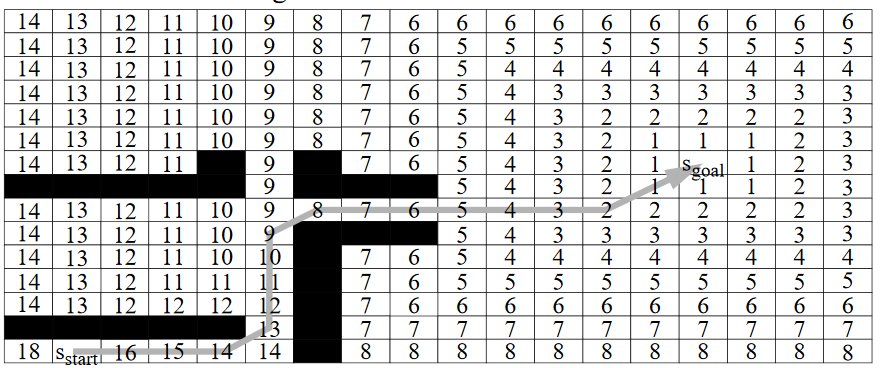
\includegraphics[width=8cm]{obr/dStarA}
		%\vspace*{4mm}
		\caption{\centering Vzdálenosti do cíle před \linebreak začátkem pohybu robota}
		\label{obr:D*a}
	\end{subfigure}%
	\begin{subfigure}{.5\textwidth}
		\centering
		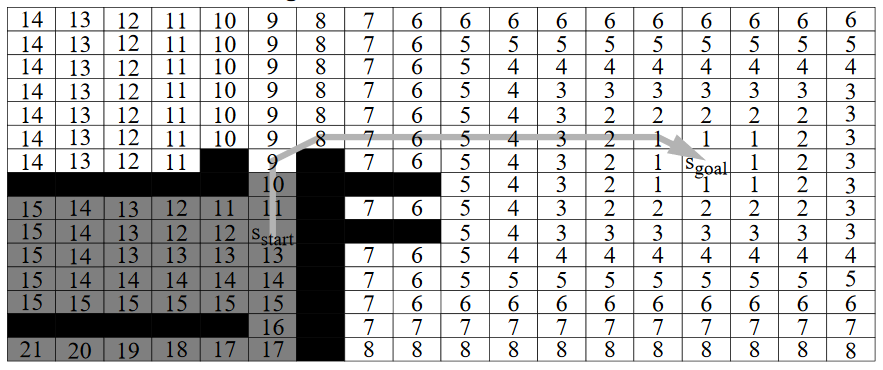
\includegraphics[width=8cm]{obr/dStarB}
		%\vspace*{4mm}
		\caption{\centering Vzdálenosti do cíle při \linebreak nalezení nové překážky}
		\label{obr:D*b}
	\end{subfigure}
	\vspace*{4mm}
	\caption{Příklad situace vyžadující replanning \cite{Koenig2002}}
	\label{obr:D*}
\end{figure}

D* Lite provádí prohledávání ve zpětném směru a tedy hodnota $g$ každé buňky odpovídá nejkratší vzdálenosti do cílového stavu. Navíc počítá odhad této vzdálenosti o krok napřed, tzv. hodnotu $rhs$. Tato hodnota je dána vztahem
\begin{equation}
	rhs(s)=\begin{cases}
	0 \qquad \text{pro } s=s_{start},\\
	\min_{s'\in Succ(s)}\left(g\left(s'\right)+c\left(s',s\right)\right) \qquad \text{jinak},
	\end{cases}
\end{equation}
kde $c(s,s')$ je cena přechodu mezi stavy $s$ a $s'$ a $Succ(s)$ jsou následovníci stavu $s$. Stav $s$ se nazývá \emph{lokálně konzistentní}, pokud $rhs(s)=g(s)$. Pokud jsou všechny stavy lokálně konzistentní, lze nalézt nejkratší cestu ze stavu $u$ do stavu $v$ zpětným chodem ze stavu $v$ tak, že vždy hledáme hranu $(s,s')$ takovou, která minimalizuje $c(s,s')+g(s')$.

Jak bylo řečeno, není efektivní počítat tyto hodnoty pro všechny stavy, proto je použita heuristická funkce, která pomáhá vybírat ty stavy, které jsou důležité pro nalezení nejkratší cesty. Podobně jako v A* algoritmu je využita prioritní fronta. Tato fronta obsahuje lokálně nekonzistentní stavy, které je potřeba přepočítat. Klíčem v této frontě je dvousložkový vektor $k(s)=[k_1(s);k_2(s)]$, kde $k_1(s)=\min(g(s),rhs(s))+h(s_{start},s)$ a $k_2(s)=\min(g(s),rhs(s))$. Složka $k_1$ odpovídá $f$ hodnotám v klasickém A* algoritmu a složka $k_2$ odpovídá hodnotám $g$. Klíče se porovnávají lexikálně, tj. $$k(s)\leq k'(s)\Leftrightarrow k_1(s)<k'_1(s)\vee (k_1(s)=k'_1(s)\wedge k_2(s)\leq k'_2(s)).$$

Pseudokód algoritmu D* Lite je popsán v algoritmech \ref{alg:DStarLiteP1} a \ref{alg:DStarLiteP2}. Hlavní funkce \texttt{Main} nejprve zavolá funkci \texttt{Initialize}, která nastaví hodnoty $rhs$ a $g$ pro všechny stavy na $\infty$. Pro cílový stav $s_{goal}$ nastaví $rhs=0$ a vloží tento stav do prioritní fronty $U$. Potom se zavolá funkce \texttt{ComputeShortestPath}, která provede hledání odpovídající A* algoritmu. Robot se poté začne pohybovat ze stavu $s_{start}$ po nejkratší cestě směrem ke stavu $s_{goal}$ (podél hrany $(s,s')$, která minimalizuje $c(s,s')+g(s')$). Pokud při pohybu zjistí, že se změnila cena některé hrany $(u,v)$, zavolá metodu \texttt{UpdateVertex}, která přepočítá hodnotu $rhs$ a klíč stavu $u$, případně jej odebere z fronty, pokud je nyní stav lokálně konzistentní, nebo jej do fronty zařadí, pokud je lokálně nekonzistentní. Poté se opět zavolá funkce \texttt{ComputeShortestPath}, která přepočítá nejkratší cestu ze stavu $s_{start}$ do stavu $s_{goal}$.

Funkce \texttt{ComputeShortestPath} vybírá k expanzi lokálně nekonzistentní stav s nejmenším klíčem. Pokud je $g(s)>rhs(s)$, nastaví hodnotu $g(s)=rhs(s)$, jinak se nastaví hodnota $g(s)=\infty$. Tím je zaručeno, že je stav lokálně konzistentní. Poté se přepočítají hodnota $g$, hodnota $rhs$ a příslušnost do prioritní fronty všech následníků stavu $s$, případně i stavu $s$ samotného pomocí funkce \texttt{UpdateVertex}. Funkce \texttt{ComputeShortestPath} expanduje stavy, dokud je stav $s_{start}$ lokálně konzistentní a klíč následujícího stavu určeného k expanzi není menší než klíč $s_{start}$. Pokud je $g_{start}=\infty$, potom neexistuje cesta ze stavu $g_{start}$ do stavu $g_{goal}$.

Jelikož je při každé změně ceny nutné přepočítávat klíče prioritní fronty, čímž by docházelo k neustálé změně pořadí v často rozsáhlé prioritní frontě, které je velmi výpočetně náročné. D* Lite tedy používá metodu převzatou z D*, díky které nemusí docházet ke změně pořadí v prioritní frontě. Při pohybu robota ze stavu $s$ do stavu $s'$, ve kterém je zjištěna změna cen přechodů, je hodnota složky $k_1$ klíčů prioritní fronty menší o maximálně $h(s,s')$, hodnota složky $k_2$ nezávisí na $h$ a je tedy nezměněna. Je tedy potřeba odečíst hodnotu $h(s,s')$ od první složky všech klíčů stavů v prioritní frontě. Protože je tato hodnota pro všechny stejná, pořadí se touto operací nezmění. Místo toho při vkládání nového stavu do prioritní fronty přičteme tuto hodnotu k první složce klíče tohoto stavu. Hodnota $h(s,s')$ se ukládá do proměnné $k_m$ a je přičtena k první složce klíče ve funkci \texttt{CalculateKey}. Je potřeba ještě upravit funkci \texttt{ComputeShortestPath} tak, aby při odebrání stavu $u$ s nejnižším klíčem $k_{old}$, přepočítala klíč tohoto stavu pomocí \texttt{CalculateKey}. Pokud je $k_{old}<\texttt{CalculateKey}(s)$, je stav $u$ opět vložen do prioritní fronty s tímto novým klíčem, jinak je tento stav expandován.

\begin{algorithm}[H]
	\caption{D* Lite}
	\label{alg:DStarLiteP1}
	\begin{algorithmic}[1]
		%\Statex Prioritní fronta $U$ má 	nasledující funkce: 
		\Statex %\hspace{\algorithmicindent}
		$U.Insert(s,k)$ -- vloží do prioritní fronty stav $s$ s klíčem $k$
		\Statex %\hspace{\algorithmicindent}
		$U.Remove(s)$ -- odstraní stav $s$ z prioritní fronty
		\Statex %\hspace{\algorithmicindent}
		$U.TopKey()$ -- vrátí nejmenší klíč z prioritní fronty ($[\infty;\infty]$ pokud je fronta prázdná)
		%\Statex \hspace{\algorithmicindent}\hspace{\algorithmicindent}
		\Statex %\hspace{\algorithmicindent}
		$U.Pop()$ -- odebere z fronty stav s nejmenším klíčem a vrátí jej\strut
		\Statex
		\Function{Initialize}{}
			\State $s_{last}\gets s_{start}$
			\State $U\gets \emptyset$
			\State $k_m\gets 0$
			\State $\forall s\in V: rhs(s)\gets g(s)\gets \infty$
			\State $rhs(s_{goal})\gets 0$
			\State $U.Insert(s_{goal},$ \Call{CalculateKey}{$s_{goal}$}$)$
		\EndFunction
		\Statex
		\Function{UpdateVertex}{$u$}
			\If{$u\neq s_{goal}$}
				\State $rhs(u)\gets \min_{s'\in Succ(u)}(c(u,s')+g(s'))$
			\EndIf
			\If{$u\in U$}
				\State $U.Remove(u)$
			\EndIf
			\If{$g(u)\neq rhs(u)$}
				\State $U.Insert(u,$ \Call{CalculateKey}{$u$}$)$
			\EndIf
		\EndFunction
	\algstore{bkbreak}
	\end{algorithmic}
\end{algorithm}

\begin{algorithm}[H]
	\caption{D* Lite (pokračování)}
	\label{alg:DStarLiteP2}
	\begin{algorithmic}[1]
	\algrestore{bkbreak}
		\Function{CalculateKey}{$s$}
		\State \textbf{return} $[\min(g(s),rhs(s))+h(s_{start},s)+k_m;\min(g(s),rhs(s))]$
		\EndFunction
		\Statex
		\Function{ComputeShortestPath}{$\,$}
			\While{$U.TopKey()<$ \Call{CalculateKey}{$s_{start}$} $ \vee\:rhs(s_{start})\neq g(s_{start})$}
				\State $k_{old}\gets U.TopKey()$
				\State $u\gets U.Pop()$
				\If{$k_{old}<$ \Call{CalculateKey}{$u$}$)$}
					\State $U.Insert(u,$ \Call{CalculateKey}{$u$}$)$
				\ElsIf{$g(u)>rhs(u)$}
					\State $g(u)\gets rhs(u)$
					\ForAll{$s\in Pred(u)$}
						\State \Call{UpdateVertex}{$s$}
					\EndFor
				\Else
					\State $g(u)\gets \infty$
					\ForAll{$s\in Pred(u)\cup{u}$}
						\State \Call{UpdateVertex}{$s$}
					\EndFor
				\EndIf
			\EndWhile
		\EndFunction
		\Statex
		\Function{Main}{$\,$}
			\State \Call{Initialize}{$\,$}
			\State \Call{ComputeShortestPath}{$\,$}
			\While{$s_{start}\neq s_{goal}$}
				\If{$g(s_{start})=\infty$}
					\State \textbf{return} failure
				\EndIf
				\State $s_{start}\gets \arg\min_{s'\in Succ(s_{start})}(c(s_{start},s')+g(s'))$
				\State move to $s_{start}$
				\State scan graph $V$ for chagned edge cost
				\If{any edge costs changed}
					\State $k_m\gets k_m+h(s_{last},s_{start})$
					\State $s_{last}\gets s_{start}$
					\ForAll{edges $(u,v)$ with changed edge costs}
						\State \Call{UpdateVertex}{$u$}
					\EndFor
					\State \Call{ComputeShortestPath}{$\,$}
				\EndIf
			\EndWhile
		\EndFunction
	\end{algorithmic}
\end{algorithm}

\subsection{Modifikace pro více robotů}
Kombinací metod plánování Local Repair A* a vyhledávání nejkratší cesty pomocí D* Lite dostáváme algoritmus použitelný pro plánování cesty více robotů. Pseudokód tohoto algoritmu můžeme vidět v algoritmu \ref{alg:LRD*Lite}.

\begin{algorithm}[H]
	\caption{Multi Agent D* Lite}
	\label{alg:LRD*Lite}
	\begin{algorithmic}[1]
		\Function{Main}{$\,$}
		\ForAll{$r\in Robots$}
			\State $r.$\Call{Initialize}{$\,$}
			\State $r.$\Call{ComputeShortestPath}{$\,$}
		\EndFor
		\State $enRoute\gets Robots$ where $r.s_{start}\neq r.s_{goal}$
		\While{$count(enRoute)>0$}
			\ForAll{$r\in enRoute$}
				\State $occupied\gets \{s\in Succ(r.s_{start})$ where $s$ is $s_{start}$ of any robot$\}$
				\State \Call{Step}{$r,occupied$}
				\State update $enRoute$
			\EndFor
		\EndWhile
		\EndFunction
		\Statex
		\Function{Step}{$r,occupied$}
			\If{$occupied$ changed since last call}
				\State $r.k_m\gets r.k_m+h(r.s_{last},r.s_{start})$
				\State $r.s_{last}\gets r.s_{start}$
				\State $r.c(u,v)\gets \infty$ if $u\in occupied\vee v\in occupied$ otherwise $1$
				\ForAll{$u\in occupied$}
					\State $r.$\Call{UpdateVertex}{$u$}
				\EndFor
				\State $r.$\Call{ComputeShortestPath}{$\,$}
			\EndIf
			\If{$g(r.s_{start})=\infty$}
			\State \textbf{return} failure
			\EndIf
			\State $r.s_{start}\gets \arg\min_{s'\in Succ(r.s_{start})}(c(r.s_{start},s')+g(s'))$
		\EndFunction
	\end{algorithmic}
\end{algorithm}

Hlavní obslužná funkce \texttt{Main} zavolá pro každého robota funkce \texttt{Initialize}\linebreak a~\texttt{ComputeShortestPath}, které jsou identické s implementací popsanou v podkapitole \ref{sec:D*Lite}. Každý robot si uchovává vlastní informace, tj. prioritní frontu, hodnoty $g,rhs,k_m$, hodnoty cen přechodů $c$ a stavy $s_{start}$ (aktuální pozice), $s_{goal}$ (cílová pozice) a $s_{last}$ (pozice poslední změny cen přechodů). Dále následuje hlavní smyčka algoritmu, kdy každý robot, který není v cílové pozici, ověří, zda-li se v jeho okolí vyskytují nějaký další robot. Pokud ano, označí dané pozice jako překážky ($occupied$). Poté se zavolá funkce \texttt{Step}, která je analogií funkce \texttt{Main} z podkapitoly \ref{sec:D*Lite}. 

Funkce \texttt{Step} nejprve ověří, zda se změnily pozice označené jako $occupied$. Pokud ano, nastaví příslušné hodnoty pro $k_m$ a $s_{last}$. Poté nastaví hodnoty cen přechodů pro stavy v $occupied$ jako $\infty$, pro ostatní jako $1$. Pro všechny stavy v $occupied$ také přepočítá hodnoty $g$, $rhs$ a příslušnost do prioritní fronty pomocí funkce \texttt{UpdateVertex}. Dále se přepočítá nejkratší cesta funkcí \texttt{ComputeShortestPath} s těmito novými informacemi. Pokud je $g(s_{start})=\infty$, cesta neexistuje, jinak se nastaví současná pozice $s_{start}$ na pozici $s'\in Succ(s)$ tak, aby se minimalizovala hodnota $c(s_{start},s')+g(s')$.

\clearpage
\chapter{Popis aplikace}
Následující kapitola se bude věnovat popisu aplikace \emph{MultiRobotSimulator}, který je výstupem praktické části této diplomové práce. Jedná se o grafické prostředí umožnující vytvářet, importovat a editovat mapy prostředí, spouštět a vyhodnocovat výsledky daných algoritmů a pomocí plug-in systému jednoduše implementovat další algoritmy pro plánování cesty více robotů.

\section{Použité technologie}
\subsubsection{C\texttt{\#}}
C\texttt{\#} (vysl. \emph{see sharp}) je moderní mnohoúčelový vysokoúrovňový objektově orientovaný programovací jazyk vyvíjený od roku 2000 firmou Microsoft zároveň s platformou \emph{.NET Framework}. Nabízí podporu pro principy softwarového inženýrství, jakými jsou např. silné typování, hlídání hranic polí, detekce použití neinicializovaných proměnných nebo automatický garbage collector. Je vhodný pro vývoj softwarových komponent vhodných pro distribuované prostředí, jak pro velká zařízení se sofistikovanými operačními systémy, tak pro malá zařízení s omezenými funkcemi. Tento programovací jazyk byl schválen normalizační organizací ECMA. \cite{ECMA} Konkrétně se jedná o multiplatformní open-source platformu \emph{.NET Core} verze 3.0. K vývoji bylo použito vývojové prostředí \emph{Visual Studio 2019}, podporující např. IntelliSense, refaktorování kódu, statickou analýzu nebo editor grafických rozhraní. \cite{MSDOCS}

\subsubsection{Windows Presentation Foundation}
Pro design grafického uživatelského rozhraní (GUI) byla zvolena technologie \emph{Windows Presentation Foundation} (WPF), která je součástí .NET Framework. Jedná se o moderního nástupce sady knihoven \emph{Windows Forms}. Základem je renderovací engine založený na vektorové grafice využívající moderních zobrazovacích zařízení, podporující hardwarovou akceleraci a technologii \emph{DirectX}. Pomocí datových vazeb umožňuje jednoduše oddělit vzhled od funkční logiky programu. \cite{MSDOCS}

\subsubsection{Stylet}
Pro zjednodušení práce s architekturou Model-View-ViewModel, která je základem WPF, byla zvolena knihovna \emph{Stylet} \cite{Stylet}, která umožňuje jednoduchou údržbu a testovatelnost kódu. Navíc obsahuje poskytovatele závislostí, tzv. IoC kontejner, jehož bylo využito při implementaci plug-in systému (podkapitola \ref{sec:plugins}).

\subsubsection{QuickGraph}
Pro reprezentaci prostředí jako grafu byla použita knihovna \emph{QuickGraph} \cite{QuickGraph}, která obsahuje generické datové struktury reprezentující neorientované a orientované grafy i některé algoritmy použitelné s těmito strukturami.

\subsubsection{High Speed Priority Queue}
Jelikož uvedené algoritmy využívají prioritní frontu, bylo použito knihovny \emph{High Speed Priority Queue} \cite{HSPQ}, která je implementovaná speciálně pro plánování cest. Tato knihovna nabízí testovanou, rychlou, generickou prioritní frontu bez závislostí na jiných knihovnách.

\section{Uživatelské rozhraní}
Cílem uživatelského rozhraní je umožnit uživatelům snadné a intuitivní používání programu. Na obrázku \ref{obr:gui} můžeme vidět hlavní okno aplikace a její popsané části.

\begin{figure}[htb]
	\begin{center}
		\includegraphics*[width=\textwidth,keepaspectratio]{obr/gui}
	\end{center}
	\caption[caption]{Hlavní okno aplikace}
	\label{obr:gui}
\end{figure}

\subsubsection{1 -- Hlavní menu}
Hlavní menu (viz obrázek \ref{obr:menu}) umožnuje uživateli vytvořit novou mapu, případně ji načíst ze souboru (formát popsán v podkapitole \ref{sec:movingAI}) nebo uložit. Při výběru možnosti vytvoření nové mapy se otevře dialog s nabídkou specifikovat požadovanou výšku a šířku (obrázek \ref{obr:newMapDialog}). Otevírání a ukládání map je zprostředkováno standardním dialogovým oknem operačního systému.

% https://tex.stackexchange.com/a/37597
\begin{figure}[htb]
	\centering
	\begin{minipage}{.5\textwidth}
		\centering
		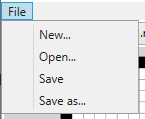
\includegraphics[height=4cm,keepaspectratio]{obr/menu}
		\vspace*{4mm}
		\caption{Hlavní menu}
		\label{obr:menu}
	\end{minipage}%
	\begin{minipage}{.5\textwidth}
		\centering
		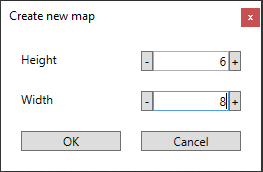
\includegraphics[height=4cm]{obr/newMapDialog}
		\vspace*{4mm}
		\caption{Dialog pro vytvoření nové mapy}
		\label{obr:newMapDialog}
	\end{minipage}
\end{figure}

\subsubsection{2 -- Záložky}
Aplikace umožňuje mít otevřeno několik map zároveň a přepínat mezi nimi pomocí záložek. Všechny funkce aplikace probíhají na aktuálně zvolené mapě.

\subsubsection{3 -- Mapa prostředí}
Prostředí je v aplikaci představováno sítí čtverců, kde bílé čtverce představují přípustné stavy a černé čtverce reprezentují překážky (nepřípustné stavy). Výchozí stavy robotů jsou zobrazeny jako zelené kruhy a cílové stavy jako kruhy červené. Stavy se stejnými čísly přísluší stejnému robotu. Stavy lze přidávat kliknutím levým tlačítkem myši v závislosti na vybraném módu na postranním panelu (4), pravým tlačítkem daný stav smažeme.

\subsubsection{4 -- Postranní panel}
Postranní panel obsahuje dvě záložky:
\begin{itemize}
	\item Editor (obrázek \ref{obr:sideEditor}) -- Obsahuje možnosti týkající se editoru mapy prostředí. Tlačítko \emph{Clear all} smaže z mapy všechny překážky a výchozí a cílové stavy robotů. Tlačítko \emph{Clear robots} smaže pouze výchozí a cílové stavy, překážky ponechá. Přepínačem \emph{Draw} je možné vybrat mód kreslení do mapy. Možnost \emph{Render graph} zobrazí v mapě hrany grafu, který reprezentuje toto prostředí. Toto zobrazení můžeme vidět na obrázku \ref{obr:renderGraph}
	\begin{figure}[htb]
		\begin{center}
			\includegraphics*[height=4cm,keepaspectratio]{obr/sideEditor}
		\end{center}
		\caption{Postranní panel -- záložka Editor}
		\label{obr:sideEditor}
	\end{figure}

\begin{figure}[htb]
\begin{center}
	\includegraphics*[height=10cm,keepaspectratio]{obr/renderGraph}
\end{center}
\caption{Zobrazení grafu v mapě (fialová)}
\label{obr:renderGraph}
\end{figure}
	
	\item Search (obrázek \ref{obr:sideSearch}) -- V této záložce si může uživatel vybrat ve výběrovníku požadovaný algoritmus. Tlačítkem \emph{Run search} se spustí hledání pomocí vybraného algoritmu. Po dokončení hledání se pod tímto tlačítkem zobrazí výsledky s těmito informacemi: počet úspěšně nalezených cest, čas inicializace algoritmu, čas potřebný k hledání a délka nejkratší cesty.
	\begin{figure}[htb]
		\begin{center}
			\includegraphics*[height=4cm,keepaspectratio]{obr/sideSearch}
		\end{center}
		\caption{Postranní panel -- záložka Search}
		\label{obr:sideSearch}
	\end{figure}
\end{itemize}

Po dokončení hledání jsou v mapě zobrazeny nalezené cesty, odlišené barevně pro lepší přehlednost. Příklad můžeme vidět na obrázku~\ref{obr:foundPaths}.

\begin{figure}[htb]
	\begin{center}
		\includegraphics*[height=10cm,keepaspectratio]{obr/foundPaths}
	\end{center}
	\caption{Zobrazení nalezených cest}
	\label{obr:foundPaths}
\end{figure}

\section{Plug-in systém}\label{sec:plugins}
Aplikace podporuje programování plánovacích algoritmů nezávisle na ostatních funkcích programu. Tohoto je dosaženo pomocí vrstvy abstrakce, jejíž schéma můžeme vidět na obrázku \ref{obr:pluginsSchema}. Uživatel ovládá aplikaci pomocí grafického rozhraní, které je obsaženo v projektu \texttt{WPF}. Programová logika je obsažena v projektu \texttt{Core}, která pomocí veřejných rozhraní (angl. interface) a abstraktních tříd provádí plánování cest robotů.

\begin{figure}[htb]
	\begin{center}
		\includegraphics*[width=15cm,keepaspectratio]{obr/pluginsSchema2}
	\end{center}
	\caption{Schéma architektury }
	\label{obr:pluginsSchema}
\end{figure}

Uživatel může naprogramovat vlastní algoritmus v jazyce C\texttt{\#}, který aplikace při startu naimportuje a je možné jej použít stejně jako zabudované algoritmy. Pro implementaci algoritmu je nutné vytvořit třídu, která dědí z abstraktní třídy \texttt{AbstractAlgo}, případně rozhraní \texttt{IAlgo}. Vlastnosti a funkce této třídy jsou následující:
\begin{itemize}
	\item \texttt{Graph} -- graf reprezentující danou mapu prostředí
	%\item \texttt{Logger} -- rozhraní umožňující zápis informací o běhu algoritmu
	\item \texttt{Name} -- název algoritmu
	\item \texttt{Robots} -- seznam robotů s danými vlastnostmi (start, cíl, nalezená cesta atd.)
	\item \texttt{Initialize()} -- funkce volaná na začátku hledání
	\item \texttt{RobotFactory(start, target)} -- funkce vytvářející instanci robota, umožňující její rozšíření uživatelem
	\item \texttt{RunSearch()} -- funkce obsahující vlastní implementaci plánovacího algoritmu
\end{itemize}

Sestavenou knihovnu \texttt{.dll} musí uživatel před spuštěním aplikace umístit do složky \texttt{plugins}, ve které se nachází i textový soubor \texttt{readme.md} s bližšími informacemi jak postupovat při implementaci.




\section{MovingAI benchmarks}\label{sec:movingAI}
Aplikace podporuje otevírání a ukládání map ve formátu, který byl zaveden Sturtevantem \cite{Sturtevant2012} v jeho článku \emph{Benchmarks for Grid-Based Pathfinding}. Jedná se o sadu mřížkových map, která je k dispozici online (\url{https://movingai.com/benchmarks/}). Tato sada obsahuje mapy z komerčních počítačových her (např. Baldurs Gate II, Warcraft III a další), mapy z městských prostředí (Berlín, Londýn, ...), mapy bludišť a další náhodně vygenerované mapy. Tyto sady jsou běžně používané ve vědeckých výzkumech pro srovnávání výsledků jednotlivých algoritmů. Příklady těchto map můžeme vidět na obrázcích~\ref{obr:AR0300SR}~a~\ref{obr:Boston}.

% TODO dávkovací režim

%\begin{figure}[htb]
%	\centering
%	\begin{subfigure}{.5\textwidth}
%		\centering
%		\includegraphics[width=6cm]{obr/AR0300SR}
%		\vspace*{4mm}
%		\caption{Mapa \texttt{AR0300SR} ze hry Baldurs Gate II}
%	\end{subfigure}%
%	\begin{subfigure}{.5\textwidth}
%		\centering
%		\includegraphics[width=6cm]{obr/Boston_0_512}
%		\vspace*{4mm}
%		\caption{Mapa \texttt{Boston\_0\_512}}
%	\end{subfigure}
%\vspace*{4mm}
%	\caption{Příklady map z MovingAI benchmarks \cite{Sturtevant2012}}
%	\label{obr:mapy}
%\end{figure}


\begin{figure}[htb]
	\begin{center}
		\includegraphics*[height=10cm,keepaspectratio]{obr/AR0300SR}
	\end{center}
	\caption[caption]{Mapa \texttt{AR0300SR} ze hry Baldurs Gate II \cite{Sturtevant2012}}
	\label{obr:AR0300SR}
\end{figure}

\begin{figure}[htb]
	\begin{center}
		\includegraphics*[height=10cm,keepaspectratio]{obr/Boston_0_512}
	\end{center}
	\caption[caption]{Mapa \texttt{Boston\_0\_512} \cite{Sturtevant2012}}
	\label{obr:Boston}
\end{figure}

%\section{Implementované algoritmy}


\clearpage
\chapter{Vyhodnocení výsledků}

\clearpage
